%%%%%%%%%%%%%%%%%%%%%%%%%%%%%%%%%%%%%%%%%%%%%%%%%%%%%%%%%%
\section{Introduction}
\label{sec:introduction}
%%%%%%%%%%%%%%%%%%%%%%%%%%%%%%%%%%%%%%%%%%%%%%%%%%%%%%%%%%

% 1. Problem Synoptic is trying to solve:
Logging is commonly used by developers to record state and behavior information 
about their systems. Logged information is useful for, among other things,
understanding and debugging programs.
Manually inspecting logs is
both tedious and challenging: logs can be enormous, spread across
multiple files, and cluttered with extraneous details. Also, often errors can
not be spotted without examining logs from multiple executions
side-by-side. These issues are exacerbated as the scale of a system grows. 

Figure~\ref{fig:motivating-log} presents a log snippet from a hypothetical
online shopping system. The site has a bug 
which is captured in the log. Unfortunately this snippet is plagued by some of the above
challenges of log analysis, making the bug difficult to spot.

% Roadmap of what's up next
In this section we first describe Synoptic, a tool designed to help developers
by inferring models of systems from their execution logs. We then introduce 
InvariMint, a tool for constructing similar models using a new 
formal languages approach.

% 2. Synoptic solution:
%%%%%%%%%%%%%%%%%%%%%%%%%%%%%%%%%%%%%%%%%%%%%%%%%%%%%%%%%%
\subsection{Synoptic}
\label{sec:synoptic}
%%%%%%%%%%%%%%%%%%%%%%%%%%%%%%%%%%%%%%%%%%%%%%%%%%%%%%%%%%

\addtocounter{footnote}{1}
\begin{figure}[t!]
   \center
   {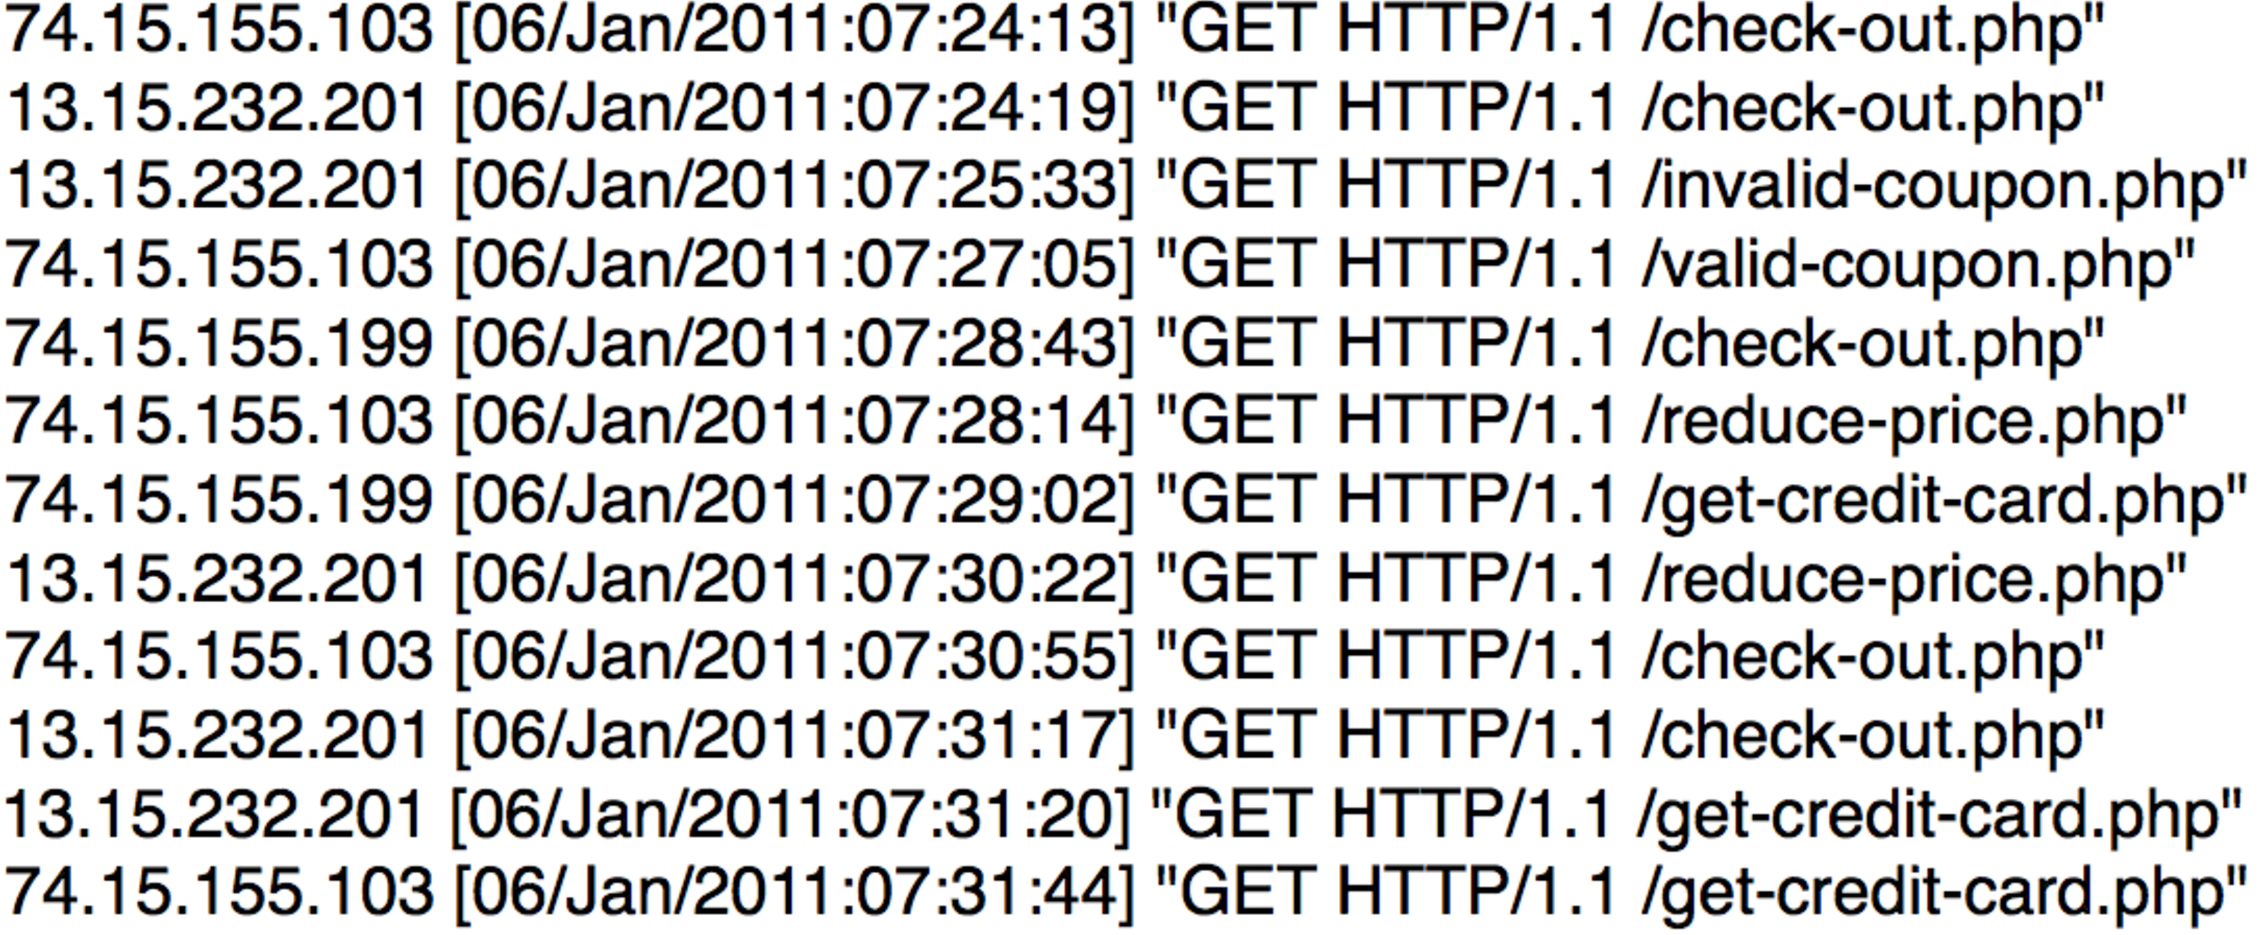
\includegraphics[width=0.95\columnwidth]{fig/motivating-log.pdf}}
   \smallskip
   \caption{Apache log snippet from an online shopping cart session - can you
   find the bug?$^{\decimal{footnote}}$}
   \label{fig:motivating-log}
\end{figure}

\footnotetext[\value{footnote}]{The user with IP address 13.15.232.201 reduces 
   the shopping cart price despite applying an invalid coupon.}

Synoptic~\cite{BeschastnikhBSSE2011} simplifies and improves the process of log
analysis 
by generating a concise model that accurately captures important properties of the
process that generated the log. The algorithm, illustrated in
Figure~\ref{fig:synop_shop}, starts with a small initial model and
performs stepwise refinement operations until the model satisfies some basic
properties inferred from the input logs. Finally Synoptic performs coarsening
operations to reduce the size of the model if possible without violating any log
properties.

In addition to execution logs, Synoptic takes as
input user-generated regular expressions that specify how to parse relevant 
behavior from the logs
as well as how to partition the input logs into individual
execution traces. The final model is an NFA that accepts
traces satisfying each of the properties inferred from the log. This includes
all of the input traces.

%%%%%%%%%%%%%%%%%%%%%%%%%%%%%%%%%%%%%%%%%%%%%%%%
\subsubsection{Invariants}
%%%%%%%%%%%%%%%%%%%%%%%%%%%%%%%%%%%%%%%%%%%%%%%%
The mined properties are invariants that capture temporal relationships
between user-specified events in the log. Synoptic mines three types of
invariants~\cite{BeschastnikhBSSE2011}:

\begin{itemize}
\item \textbf{a Never Followed by b}: Whenever the event
type $a$ appears, the event type $b$ never appears later in the same trace.

\item \textbf{a Always Followed by b}: Whenever the event
type $a$ appears, the event type $b$ always appears later in the same trace.

\item \textbf{a Always Precedes b}: Whenever the event
type $b$ appears, the event type $a$ always appears before $b$ in the same
trace.
\end{itemize}

These have been shown to capture the most commonly used patterns in formal
specification~\cite{dwyer_spec_patterns_1999}.

%%%%%%%%%%%%%%%%%%%%%%%%%%%%%%%%%%%%%%%%%%%%%%%%
\subsubsection{Model Inference}
\label{synop_inference}
%%%%%%%%%%%%%%%%%%%%%%%%%%%%%%%%%%%%%%%%%%%%%%%%
Synoptic begins with an initial model in which every instance of event type
$a$ is merged into a single partition and there exists an edge between the
partitions for $a$ and $b$ if an event $b$ ever immediately
followed an event $a$ in any input trace. The model is then refined by splitting
partitions until it satisfies each of the mined invariants. 

Splitting a
partition involves dividing that partition's event instances into two sets that
become distinct partitions of the same event type.
Refinement is a costly procedure because on each iteration Synoptic enumerates counter
example paths through the model for each unsatisfied invariant. From these, one
partition is selected to be divided such that at least one counter example is eliminated.
To make this decision, Synotic refers to the input logs to track the
source of event instances and to ensure that every input trace is accepted by
the final model.

After the model satisfies each invariant, there is an additional coarsening step
which seeks to minimize the model by merging partitions without 
un-satisfying any invariants.

The final model is an NFA state machine that accepts possible execution
sequences of the system inferred from the input logs, including all of the input traces. Developers
report finding it easy to find buggy behavior using these models.\cite{BeschastnikhBSSE2011}.

%Transition paragraph.
We next present InvariMint, which employs a novel technique for generating
similar graphical log summaries. 

\begin{figure}
   \center
   {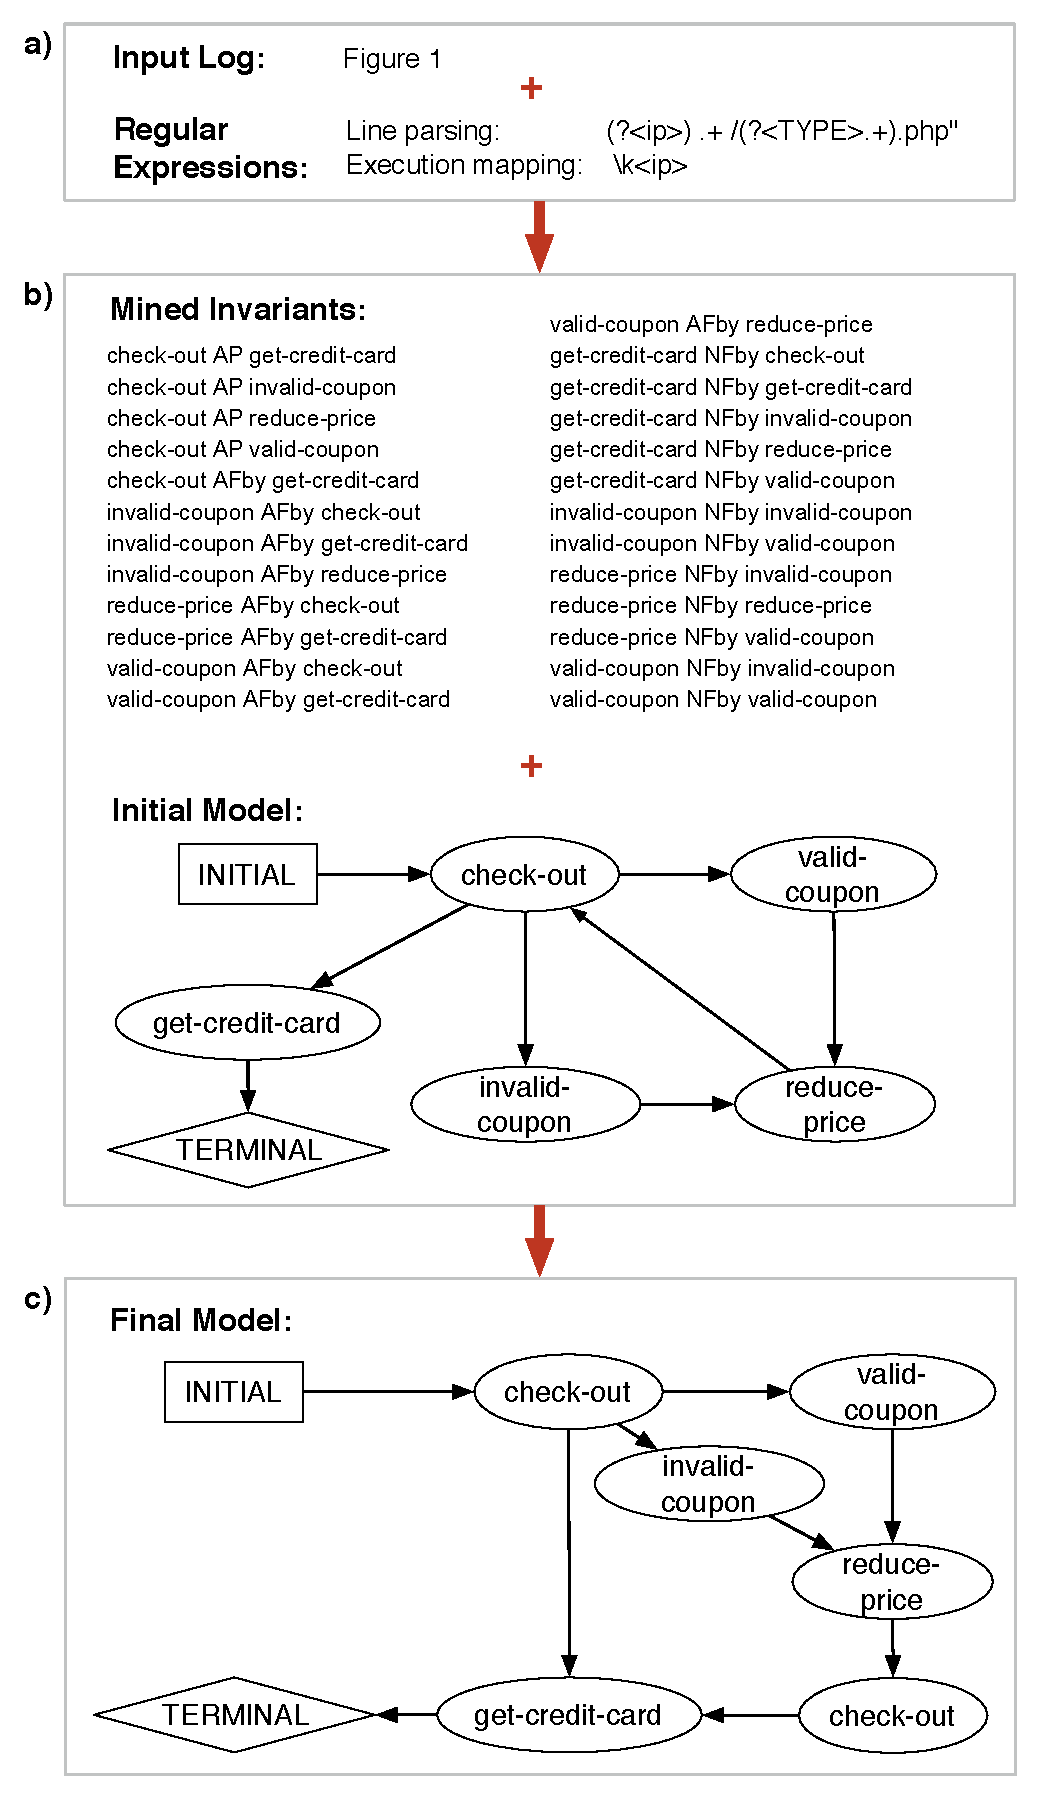
\includegraphics[width=0.95\columnwidth]{fig/shopping_cart.pdf}}
   \smallskip
   \caption{The Synoptic process for the log snippets in
   Figure~\ref{fig:motivating-log}. The user-provided regular expressions, (a),
   tell Synoptic how to parse interesting events from the input log and how to divide the log into
   individual traces of execution. Here traces are distinguished by IP address
   and Synoptic models client behavior during the shopping cart session.
   Starting from
   a compact initial model and the set of invariants mined from the input logs, (b), Synoptic 
   infers a model of the system by iteratively satisfying each unsatisfied
   invariant (e.g. valid-coupon Never Followed by valid-coupon).
   The final model, (c), accepts only traces satisfying \emph{all} of the
   invariants.}
   \label{fig:synop_shop}
\end{figure}
% 4. Describe InvariMint and why it is better:
%%%%%%%%%%%%%%%%%%%%%%%%%%%%%%%%%%%%%%%%%%%%%%%%%%%%%%%%%%
\subsection{A formal languages perspective}
%%%%%%%%%%%%%%%%%%%%%%%%%%%%%%%%%%%%%%%%%%%%%%%%%%%%%%%%%%

Another way to frame Synoptic is in terms of the language of
traces accepted by the final model.
All Synoptic models, including the intermediate ones,
accept the input traces.
Further, by construction, the final Synoptic model accepts only those
traces that satisfy the mined invariants.

The language acceptance perspective motivates a new approach for deriving
Synoptic--style models. In this approach, we generate a minimal
deterministic finite automaton (DFA) that accepts the
intersection of the languages accepted by DFAs corresponding to each log
invariant.

To evaluate this technique, we built InvariMint. InvariMint, like Synoptic,
accepts as input execution logs and regular expressions, and mines 
temporal invariants. Rather than a series of refinement and
coarsening steps, however, InvariMint replaces the model inference engine in
Synoptic with a series of DFA operations. First InvariMint creates a DFA 
for each invariant. Then InvariMint intersects these DFAs to generate a model that
accepts only traces satisfying all of the invariants.
This model can be efficiently
reduced to the
most compact representation possible that preserves the
language of the intersected model by applying DFA minimization.

InvariMint processes the input logs only once to mine invariants.
By using an inference algorithm that avoids referencing the input logs, InvariMint
generates minimal models more efficiently than Synoptic.

